\ifEnglish
%%%%%%%%%%%%%%%%%%%%%%%%%%%%%%%%%%%%%%%%%%%%%%%%%%%%%%%%%%%

\section{Introduction}


\begin{frame}[standout]
    There is a certain valuable art of thinking ...
    % TODO. Also: rework
\end{frame}



\begin{frame}[c]{Statistical Bias}
    Example: Urn with 70 white and 30 red balls. \newline
    \newline \pause
    You take 10 out.
\end{frame}

\begin{frame}[c]{Cognitive Biases}
    Example:\pause 
    \newline \pause
    (Confirmation Bias)
\end{frame}

%%%%%%%%%%%%%%%%%%%%%%%%%%%%%%%%%%%%%%%%%%%%%%%%%%%%%%%%%%%
\else
%%%%%%%%%%%%%%%%%%%%%%%%%%%%%%%%%%%%%%%%%%%%%%%%%%%%%%%%%%%

\section{Einführung}

\begin{frame}[standout]
    Es gibt eine gewisse wertvolle Art zu denken ...
    % welche nicht in Schulen gelehrt wird. Oder überhaupt irgendwie
    % systematisch. Manchmal ist sie absorbiert worden, aus Büchern, aus
    % Artikeln, vorgehensweisen und Denkweisen von anderen Menschen. Meistens
    % hat diese Art zu Denken etwas mit Wissenschaft zu tun, mit der
    % Experimentellen Methode. Der teil, bei dem die Realität konfrontiert,
    % anstatt sich dinge auszudenken. Der teil, bei dem man 'Oops' sagt und
    % eine Theorie aufgibt wenn sie nicht von Beweisen gestützt wird.
    % 
    % Aber diese Art zu Denken ist mehr als das. Tiefer und allgemeiner als
    % eine Brille, die man wieder auszieht wenn man das Labor verlässt. Sie ist
    % anwendbar im Täglichen Leben, wenn auch schwieriger und subtiler. Aber
    % wenn man nicht 'Oops, das geht wohl anders' sagen kann wenn etwas
    % offensichtlich schief läuft, bliebt keine andere Wahl als sich selbst in
    % den Fuß zu schießen.
    % 
    % Wir alle kennen Jemanden der so handelt. Und irgendwo, auch wenn man
    % eigentlich nicht daran denken möchte, handelt man ja doch irgendwo
    % genauso. Es wäre schön wenn es einen anderen Weg gäbe.
    % 
    % Den stelle ich euch nun also vor, Ich hoffe ihr nehmt zumindest irgendwas
    % daraus mit.
\end{frame}


\begin{frame}[c]{Beispiel}
    \pause
    Urne mit 70 Weißen und 30 Roten bällen. \newline
    \newline \pause
    Man zieht 10. \newline
    \newline \pause
    Was, wenn die Weißen Kugeln schwerer sind? \newline
    \newline \pause
    $\mapsto$ Stastische Vorurteile
\end{frame}


\begin{frame}[c]{Kognitive Vorurteile - Erklärung}
    \pause
    Beispiel: Ich bin unbeliebt. \newline
    % erzählen: man sieht die welt so wie man sie sehen möchte, sucht
    % hauptsächlich nach bestätigungen und übergeht gegenteiliges
    \newline \pause
    Hier helfen mehr Daten selten.
\end{frame}


% \begin{frame}[c]{Kognitive Vorurteile - Wie viele gibt es}
%     \centering
%     % trim = l b r t
%     \includegraphics[width=\textwidth, clip=true, trim = 300mm 370mm 300mm 370mm]{cogbias}
% \end{frame}


\begin{frame}[c]{Liste der Kognitiven Vorurteile}
    \centering
    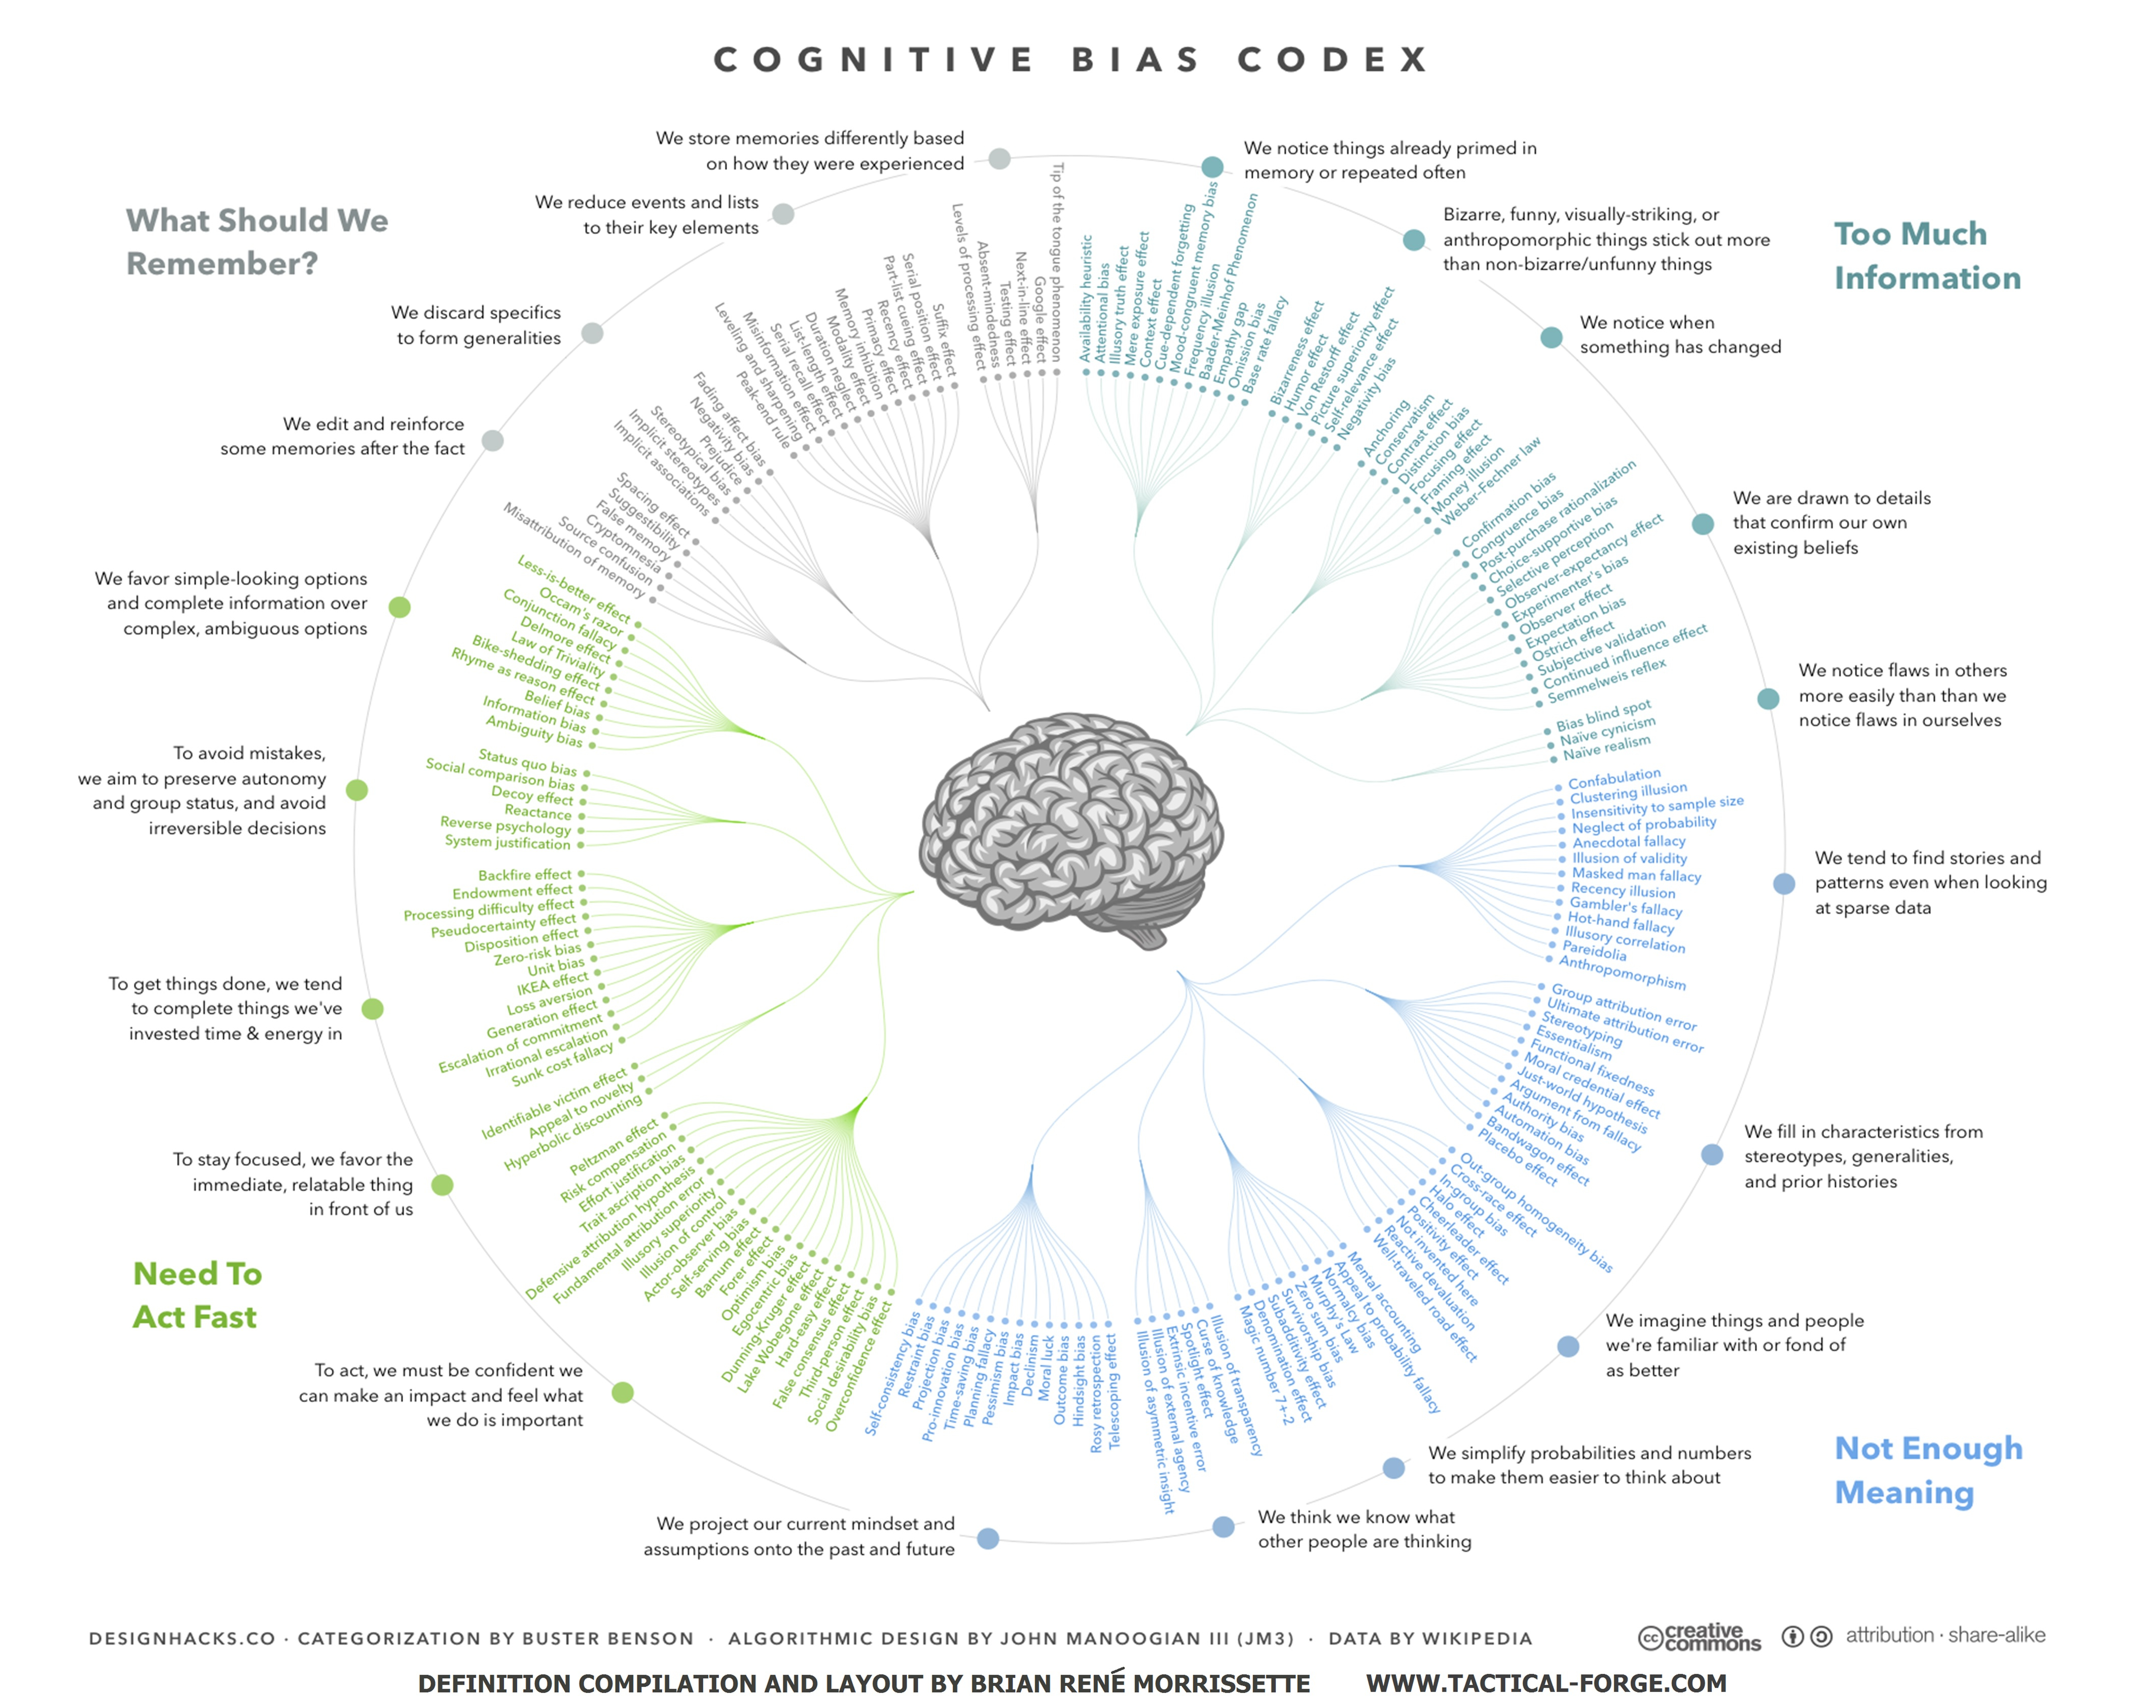
\includegraphics[width=\textwidth]{cogbias_0}
\end{frame}

\begin{frame}[c]{Kognitive Vorurteile - Wie viele gibt es II}
    \centering
    \includegraphics[width=0.9\textwidth, clip=true]{cogbias}
\end{frame}

\begin{frame}[c]{Kognitive Vorurteile - Was soll man sich merken?}
    \centering
    % trim = l b r t
    % Tip of the Tongue, Google effekt
    % \includegraphics[width=\textwidth, clip=true, trim = 600mm 1450mm 900mm 5mm]{cogbias}
    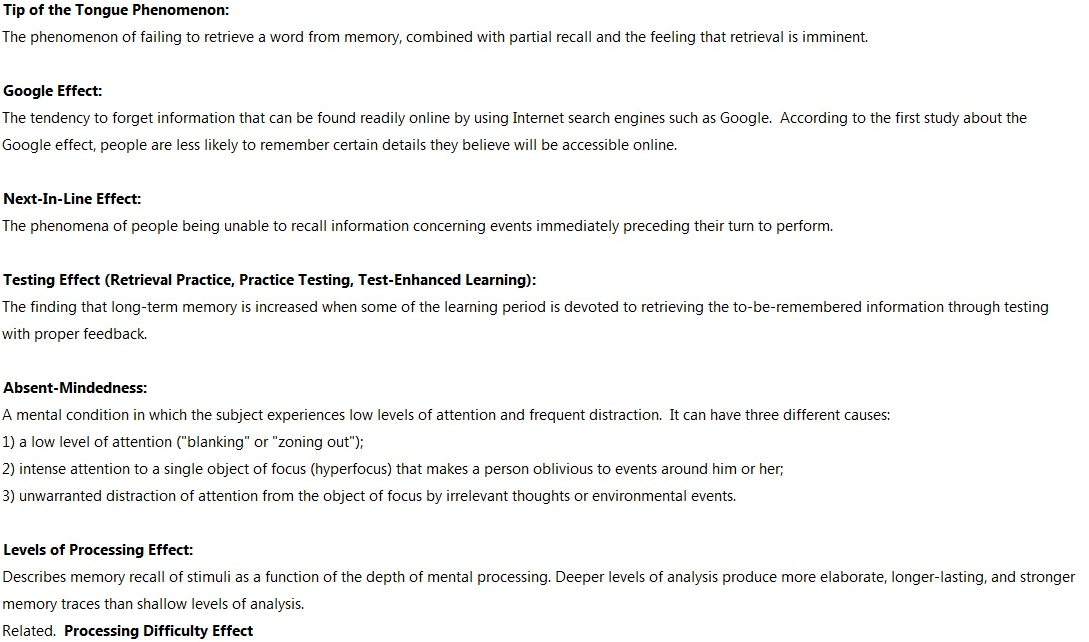
\includegraphics[width=\textwidth]{cogbias_1}
\end{frame}

\begin{frame}[c]{Kognitive Vorurteile - Schnelle Reaktionen}
    \centering
    % trim = l b r t
    % Optimism Bias, Dunning-Kruger
    % \includegraphics[width=\textwidth, clip=true, trim = 900mm 100mm 600mm 1350mm ]{cogbias}
    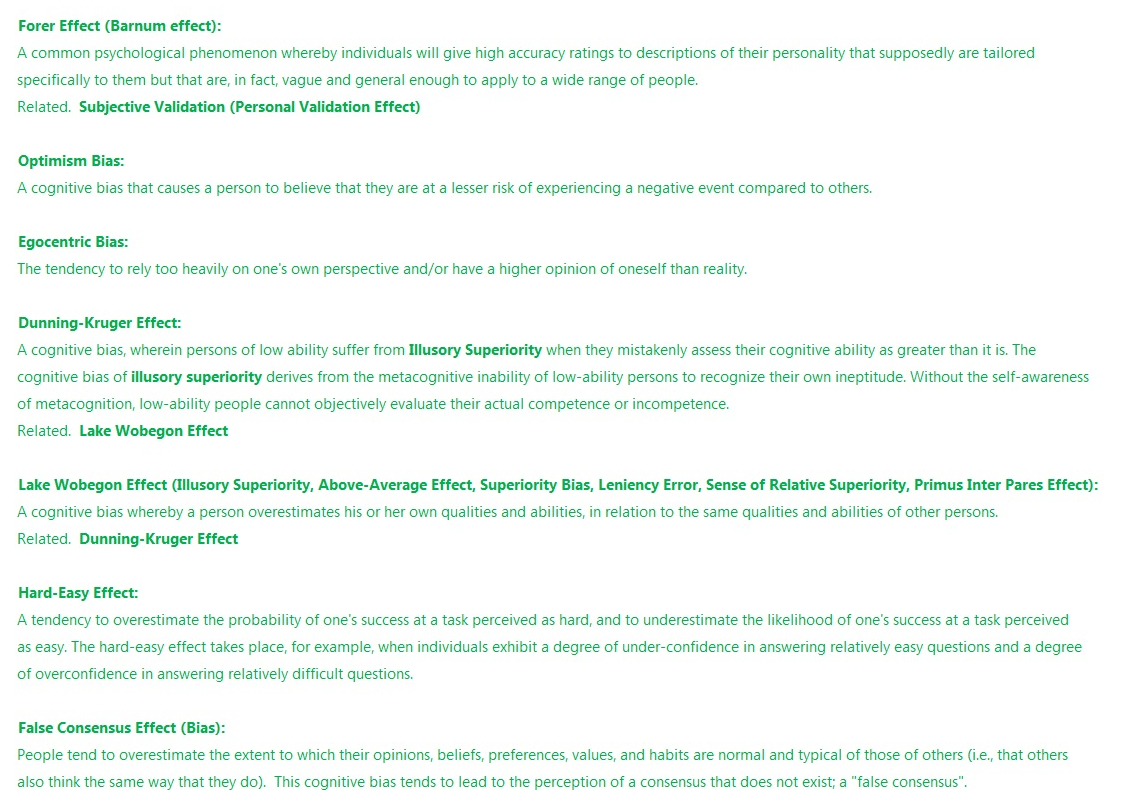
\includegraphics[width=\textwidth]{cogbias_2}
\end{frame}

\begin{frame}[c]{Kognitive Vorurteile - Zu wenig Bedeutung}
    \centering
    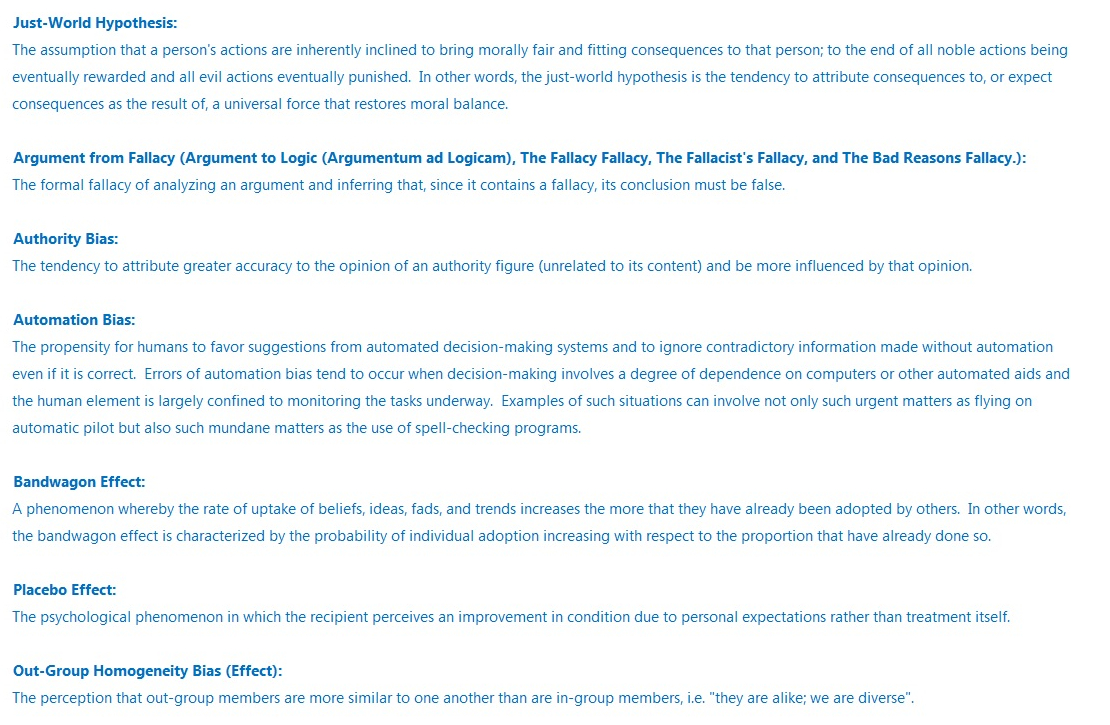
\includegraphics[width=\textwidth]{cogbias_3}
\end{frame}

\begin{frame}[c]{Kognitive Vorurteile - Zu wenig Bedeutung II}
    \centering
    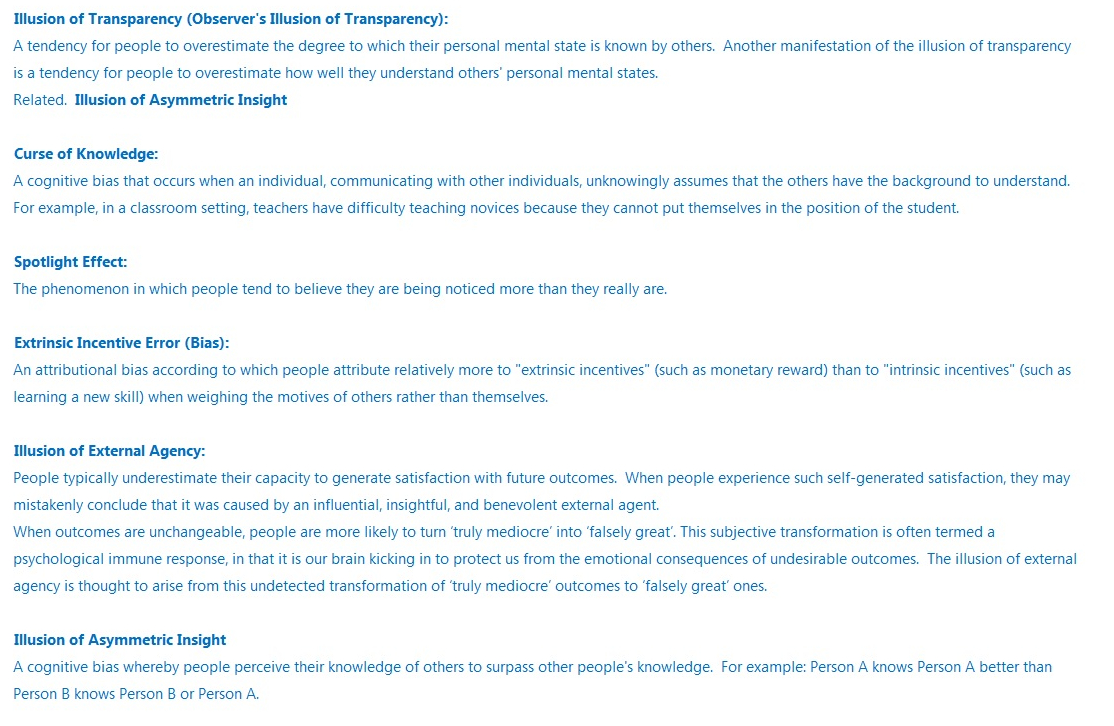
\includegraphics[width=\textwidth]{cogbias_4}
\end{frame}


% Rheinfolge der Bias-Gruppen:
% Angefangen mit Tip of the Tongue, Google effekt (mitte oben)
% Dann: Optimism Bias, Dunning-Kruger (mitte unten)
% Dann: Self-Serving Bias (links unten)
% Dann: Illusion of Transparency, Curse of Knowledge (unten mitte rechts)



\begin{frame}[c]{Kognitive Vorurteile - Zusammenfassung}
    \begin{itemize}
%        \pause
        \item Verzerren Überzeugungen
        \pause
        \item Verzerren Entscheidungsprozesse
        \pause
        \item Verzerren Weltsicht \newline
        \pause
    \end{itemize}
    Wie also gute Entscheidungen treffen? \newline \pause
\end{frame}


\begin{frame}[standout]
    Rekalibrierung des Gehirns!
\end{frame}


\begin{frame}[c]{Rekalibrierung ...}
    $...$ bzw. den Weg dorthin wollen wir nun also als Rationalität bezeichnen.
    % \newline \newline \pause
    % Achtung: Es gibt keinen einen richtigen weg, nur ein paar um {\em weniger viel} Falsch zu liegen.
\end{frame}


\begin{frame}[c]{Was ist ein Rationalist?}
    % TODO: ein paar Memes mit Spock <Hollywood-Rationalität> etc.
    Das ist es nicht. \newline
    Eigentlich ist es nur $...$ ein Systematischer Denker.
    Eigentlich ist es nur $...$ ein Strukturierter Denker.
    Eigentlich ist es nur $...$ ein Strukteren-Optimierer.
\end{frame}


\begin{frame}[c]{Rationales Denken}
    \pause
    Wird unterschieden in zwei Kategorien: \newline
    \pause
    \begin{itemize}
        \item Epistemische Rationalität \pause
        \item Instrumentalisierte Rationalität
        \newline
    \end{itemize}
    \pause
    Wir werden uns von beidem ein wenig anschauen.
\end{frame}


\begin{frame}[c]{Übliche Kognitive Vorurteile}
    nach Twersky und Kahnemann, Tennisspieler, schüchterner Verkaufsmann vs Büchereiaufsicht, sunk cost fallacy, confirmation bias, conjunction fallacy
\end{frame}


\begin{frame}[c]{Rationalität als Kampf gegen Kognitive Vorurteile}
    % TODO: List of Cognitive Biases
    Bild: List of Cognitive Biases
\end{frame}


\begin{frame}[c]{Wiederholung}
    \begin{itemize}
        \pause
        \item Statistische Vorurteile
        \pause
        \item Verzerrte Wahrnehmung
        \pause
        \item Rekalibrierung
        \pause
        \item Arten von Rationalität
        \pause
        \item {\em viele} Kognitive Vorurteile
    \end{itemize}
\end{frame}


%%%%%%%%%%%%%%%%%%%%%%%%%%%%%%%%%%%%%%%%%%%%%%%%%%%%%%%%%%%
\fi
